%%%%%%%%%%%%%%%%%%%%%%%%%%%%%%%%%%%%%%%%%%%%%%%%%%%%%%%%%%%%%%%%%%%%%%%%%%%%
%%%                    REQUIRED PACKAGES FOR DOCUMENT                    %%%
%%%%%%%%%%%%%%%%%%%%%%%%%%%%%%%%%%%%%%%%%%%%%%%%%%%%%%%%%%%%%%%%%%%%%%%%%%%%
\documentclass[12pt]{article}
\usepackage[T1]{fontenc}
\usepackage[english]{babel}
\usepackage[square,sort,comma,numbers]{natbib}
\usepackage{url}
\usepackage[utf8x]{inputenc}
\usepackage{amsmath}
\usepackage{graphicx}
\graphicspath{{images/}}
\usepackage{parskip}
\usepackage{fancyhdr}
\usepackage{vmargin}
\usepackage{xcolor}		
\usepackage{listings}									% For inserting code
\usepackage{sty/tikz-uml}  								% For UML diagrams
								
% Listing -> Code
\renewcommand{\lstlistingname}{Code}
% List of Listings -> List of Codes
\renewcommand{\lstlistlistingname}{List of \lstlistingname s}
%%%%%%%%%%%%%%%%%%%%%%%%%%%%%%%%%%%%%%%%%%%%%%%%%%%%%%%%%%%%%%%%%%%%%%%%%%%%
%%%                       DOCUMENT SETUPS (AESTHETIC)                    %%%
%%%%%%%%%%%%%%%%%%%%%%%%%%%%%%%%%%%%%%%%%%%%%%%%%%%%%%%%%%%%%%%%%%%%%%%%%%%%
\title{Laboratory 2: Authentication}					% Title
\author{Román Cárdenas}									% Author
\date{\today}											% Date

% Make title etc. accessible from any part of the document
\makeatletter
\let\thetitle\@title
\let\theauthor\@author
\let\thedate\@date
\setlength{\@fptop}{0pt}
\makeatother

% Set margins
\setmarginsrb{3 cm}{2.5 cm}{3 cm}{2.5 cm}{1 cm}{1.5 cm}{1 cm}{1.5 cm}

% Set header
\pagestyle{fancy}
\fancyhf{}
\rhead{\theauthor}
\lhead{\thetitle}
\cfoot{\thepage}

% For non-numbered lists to use dashes (-)
\renewcommand{\labelitemi}{\textendash}
%%%%%%%%%%%%%%%%%%%%%%%%%%%%%%%%%%%%%%%%%%%%%%%%%%%%%%%%%%%%%%%%%%%%%%%%%%%%
%%%                            DOCUMENT STARTS                           %%%
%%%%%%%%%%%%%%%%%%%%%%%%%%%%%%%%%%%%%%%%%%%%%%%%%%%%%%%%%%%%%%%%%%%%%%%%%%%%  
\begin{document}
\begin{titlepage}
	\centering
    \vspace*{0.5 cm}
    
\includegraphics[scale = 0.05]{DTU.png}\\[1.0 cm]	        		% University Logo
    \textsc{\LARGE Technical University of Denmark}\\[2.0 cm]	% University Name
	\textsc{\Large 02239}\\[0.5 cm]				        						% Course Code
	\textsc{\large Data Security}\\[0.5 cm]				        				% Course Name
	\rule{\linewidth}{0.2 mm} \\[0.4 cm]
	{ \huge \bfseries \thetitle}\\
	\rule{\linewidth}{0.2 mm} \\[1.5 cm]
	
	\begin{minipage}{0.4\textwidth}
		\begin{flushleft} \large
			\emph{Author:}\\
			\theauthor
		\end{flushleft}
	\end{minipage}~
	\begin{minipage}{0.4\textwidth}
		\begin{flushright} \large
			\emph{Student Number:} \\
			s182004									% Your Student Number
		\end{flushright}
	\end{minipage}\\[2 cm]
	
	{\large \thedate}\\[2 cm]
	\vfill
\end{titlepage}
\tableofcontents
\listoffigures
% \listoftables
\lstlistoflistings
\pagebreak
\section{Introduction}\label{sec:intro}
	This report addresses the problem of authentication in client/server applications.\\ \\
The Authentication Laboratory addresses this problem by designing and implementing a simple password-based authentication mechanism for a print server application which must authenticate all requests from the client.
The following assumptions were considered:
\begin{itemize}
	\item The issue of enrolment of users is not considered: authentication data structures were populated beforehand.
	\item Secure communication between client and server is ensured by other means. Confidentiality and integrity are supposed to exist between clients and server. This assumption also applies to the communication between the server and the password storage entity.
\end{itemize}
The design and implementation of the print server considered the problems of password storage, password transport and password verification.
\begin{itemize}
	\item \textbf{Password storage:} Three different scenarios are discussed: passwords stored in a system file, passwords stored in a public file with use of cryptography and passwords stored in a database management system.
	\item \textbf{Password transport:} both individual request authentication and session authenticated problems are discussed.
	\item \textbf{Password verification:} taking into account the password storage strategy, a password verification method is chosen.
\end{itemize}
The proposed solution is based on individual request authentication. The password storage is on a database management system. Password is stored hashed in order to avoid security threads. The system uses the SHA-256 algorithm for digesting the passwords. It also uses salts to prevent from rainbow tables attacks in case of the users' information is leaked to the outside.

The print server software has been proven to process clients request only if the request is successfully authenticated, as expected in the laboratory requirements.
	\pagebreak
\section{Authentication}\label{sec:auth}
	\textit{Electronic authentication}, as defined in \cite[p. 1]{Burr2013}, is "the process of establishing confidence in user identities electronically presented to an information system". In the case of client/server applications, authentication addresses the mechanisms that a given server-based application needs to perform in order to identify all the incoming requests as requested by a given client and verify that this client has access or permission to use the requested resource.\\
In password-based authentication systems, a user enters some identification, such as username, which can be available to the public as it does not provide the real protection. The protection system then requests a password from the user. If the password matches the one on file for the user, he/she is authenticated and access is allowed. Otherwise, the system does not grant access to the user.
\subsection{Password storage}\label{subsec:pwdstore}
The server must access to all clients' passwords, or at least modified information that makes possible for the server to match a password with a given user.\\
At the same time, users demand that their passwords keep safe, ensuring that knowing the password is enough for authenticating a client. In this report, three password storage mechanisms are analysed.
\subsubsection*{Passwords stored in a system file}\label{subsubsec:pwdstore1}
In this scenario, the usernames and their respective passwords are stored in the server's local host. The operating system protection mechanisms are the ones in charge of keeping users' information safe.\\
The only advantage of this solution is its simplicity: in order to verify a user's identity, the server has just to read a local file and check if the password matches with the one given by the client.\\
However, several drawbacks lead us to reject this solution:
\begin{itemize}
	\item \textit{Entries order:} in the case of a system with a high number of users, the server will spend a lot of time just reading the file until it finds the entry that corresponds to the client that is currently requesting a service.
	\item \textit{Sharing password storage mechanisms with other services:} As the file that gathers all the users' information is kept safe by the local host system, it will be impossible to share the password storage system with others servers unless they run on the same host.
	\item \textit{Not enough secure:} the system administrator should be constantly checking if the current version of the OS is secure, and if not, update it to the latest version. Even if the system is rigorously updated, this does not reduce this security threat to zero.
\end{itemize}
\subsubsection*{Passwords stored in a public file with use of cryptography}\label{subsubsec:pwdstore2}
This second scenario proposes that the file with all the users' information can be accessed by anyone. However, by using cryptography, all the content will be kept secure.\\
With this system, security is achieved. However, as the storage is done in a file, performance issues are still there. Also, the file will only be readable for those processes able to decrypt it. In order for many servers to read this file and share the password management system, all the servers must know the secret key required for decrypting its content. A shared secret key is a potential security threat, as \textit{keeping the secret secret} becomes a difficult task.
\subsubsection*{Password stored in a database management system}\label{subsubsec:pwdstore3}
In this case, a database server stores all users information. The application server request only the necessary information for checking one client's authenticity.\\
Communication between server and DBMS is assumed to be confidential by means of encryption, ensuring the solution's security.\\
With this architecture, several servers can share the password storage system, they only need to be able to establish a secure channel with the DBMS.\\
Finally, as information is stored in relational databases instead of files, the time required for verifying one user's authenticity will be lower in than previous cases.
\subsection{Password transport}\label{subsec:pwdtrans}
Two password transport scenarios are discussed: individual request authentication and authenticated sessions.
\subsubsection*{Individual request authentication}\label{pwdtrans1}
In this scenario the user authenticates his/her identity in each request: username and password should be sent \textbf{always}. This may be inconvenient, as there are more chances for network sniffers to get someone's password. However, as confidentiality is assumed between client and server, this should not be an issue to take into account for this laboratory session.
\subsubsection*{Authenticated sessions}\label{pwdtrans2}
With authenticated sessions, the user calls a specific method to authenticate his/her identity (login). If the user is authenticated, he/she receives a ticket that only he/she knows (which means that this new ticket also authenticates the user). After this, he/she will not send the password again, but the ticket.\\
If the protocol used for login can ensure that the ticket is only known by a given user, the use of sessions can prevent the user for sending his/her password in the clear, reducing security threats.\\\\
As confidentiality is supposed between client and server, this password transport is not taken into account for the service implementation.
\subsection{Password verification}\label{subsec:pwdverif}
Password verification is described for a scenario with an external DBMS for password storage mechanisms and individual request authentication.\\
The DBMS will hold a table that gathers the username, salt and the hashed password for each user. Under no circumstances is recommended storing passwords in plain text; hashing them prevents authentication threats in case user information is leaked to the outside.The hashing method is as follows:
\begin{itemize}
	\item When introducing a new user with a given password, the server will compute a 20 byte-random string (salt). The salt is different for each user.
	\item The salt is prepended to the user's chosen password and hashed.
	\item The DBMS holds, for each user, the username, the salt and the hashed salt and password.
\end{itemize}
Clients include their username and password in each request. The server will ask the DBMS for the salt and hashed salt and password that belongs to the username provided in the request. After prepending the salt to the password sent by the client and hashing them, if the result coincides with the DBMS response, the server will conclude that the client is authenticated as the user, and process the request. Otherwise, the request will be rejected.
	\pagebreak
\section{Design and Implementation}\label{sec:design}
	\subsection{Identified entities in the proposed solution}
\begin{itemize}
	\item \textbf{Client:} sends requests to the print server. In order to get the desired action done, the client must send with each request a valid username and its correspondent password.
	\item \textbf{Server:} controls the printer and receives all the requests from the clients. For each request, the server must verify that the client is authenticated. In order to do that, information related to the user that asks for a service is requested to the DBMS. If the username and hashed password match with the information stored in the DBMS, the server will execute the user request.
	\item \textbf{Database management system:} stores all the information regarding the users that can make use of the printing service. For each user, the database holds the username, the salt used for hashing the password and the hashed salt and password.\\
		The database model for this laboratory is represented in \textit{Figure \ref{fig:dbmodel}}.
\end{itemize}
\begin{figure}[hb]
	\centering	
	\begin{tikzpicture}[scale=1.2]
	\umlclass[fill=white]{users}{\textbf{id:} integer <PK>}{\textbf{name:} text NOT NULL UNIQUE\\\textbf{salt:} text NOT NULL\\\textbf{password:} text NOT NULL}
\end{tikzpicture}
	\caption{Implemented database model}
	\label{fig:dbmodel}
\end{figure}
\subsection{Print server interface}
For implementing the server, Java Remote Method Invocation (RMI) is used.\\
The interface follows the one described in the laboratory statement. However, as authentication is to be performed for each invocation, the fields \textit{username} and \textit{passwords} are added. \textit{Code \ref{lst:interface}} gathers the print service interface. 
\begin{lstlisting}[language=Java, caption=Print service interface, basicstyle=\scriptsize, label={lst:interface}]
String print(String filename, String printer, String username, String password);
List<String> queue(String username, String password);
String topQueue(int job, String username, String password);
void start(String username, String password);
void stop(String username, String password);
void restart(String username, String password);
String status(String username, String password);
String readConfig(String parameter, String username, String password);
void setConfig(String parameter, String value, String username, String password);
\end{lstlisting}
\subsection{Service architecture}
\textit{Figure \ref{fig:arch}} shows the simplified print service architecture. As depicted, there is no direct communication between users and DBMS.\\
\begin{figure}[hb]
	\centering
	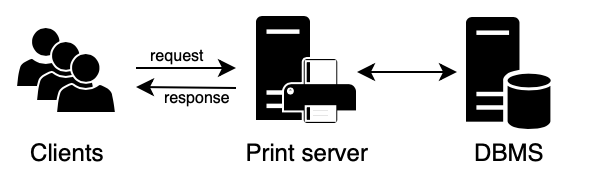
\includegraphics[width=10cm]{images/architecture}
	\caption{Print service architecture}
	\label{fig:arch}
\end{figure}
\\The sequence diagram depicted in \textit{Figure \ref{fig:seqdiag}} explains how the system functions. The client request is only processed if the authentication process successes. Otherwise, the server will respond with a deny of service message.
\begin{figure}[h]
	\centering	
	\begin{tikzpicture}[scale=1.2]
	\begin{umlseqdiag}
		\tikzumlset{font=\scriptsize}
		\umlactor[no ddots, fill=white]{client}
		\umlobject[no ddots, fill=white]{print server}  
		\umldatabase[no ddots, fill=white]{dbms} 
		\begin{umlcall}[op={request,username,password}]{client}{print server}	
			\begin{umlcall}[op={get(username)},return={salt, hash}]{print server}{dbms}	
			\end{umlcall}
			\begin{umlcall}[op={digest=SHA256(salt+password)}]{print server}{print server} 
			\end{umlcall} 
			\begin{umlfragment}[type=alt, label={digest==hash}, inner xsep=15] 
				\begin{umlcall}[op={process request}]{print server}{print server} 
				\end{umlcall} 
				\begin{umlcall}[op={response}]{print server}{client} 
				\end{umlcall} 
				\umlfpart[digest!=hash] 
				\begin{umlcall}[op={access denied}]{print server}{client} 
				\end{umlcall} 
			\end{umlfragment} 
			\end{umlcall}
	\end{umlseqdiag}
\end{tikzpicture}
	\caption{Print service sequence diagram}
	\label{fig:seqdiag}
\end{figure}
\subsection{Print service developed software}
This section summarises all the Java classes developed for this laboratory.\\
For implementing the DBMS, the SQLite database engine has been chosen. The JAR package \textit{sqlite-jdbc} needs to be added to the project before running the code.
\begin{itemize}
	\item \textbf{crypto.HashGenerator:} Java class for generating salts and hashing Strings. The encryption algorithm for hashing the passwords that has been selected is SHA-256. This algorithm, used together with salt, is secure enough for a simple print server.
	\item \textbf{db.DataBaseManager:} Java class for interacting with a SQLite database. User authentication is done in the method \textit{checkUserAuth}. In case there is no prior database, executing its main method a new database will be populated with the users \textit{user1} and \textit{user2}. For simplicity, their passwords will coincide with their username.
	\item \textbf{clientserver.PrintService:} print service interface for RMI application.
	\item \textbf{clientserver.PrintServant:} Java class with all the print services implementation. Before proceeding to execute clients' requests, all the classes will check user authenticity.
	\item \textbf{clientserver.PrintServer:} Java class that implements the RMI server. Run this class for launching the print service.
	\item \textbf{clientserver.Client:} Java class that implements a client. Running this class, the process will prove all the RMI methods, as well as try to access to services with both valid and invalid usernames and passwords.
\end{itemize}
	\pagebreak
\section{Evaluation}\label{sec:eval}
	The software developed for the print server prints logs on the output console different information regarding the print server functioning. By following these logs, it is easy to demonstrate that no request is processed before the user is successfully authenticated.
\begin{lstlisting}[language=Java, caption={RMI function example}, label={lst:function}, basicstyle=\scriptsize]
public String status(String username, String password) throws RemoteException{
	System.out.println("REMOTE CALL: status");
    if (user_authenticated(username, password)) {
     	System.out.println("   Processing request");
        return String.valueOf(this.status);
    } else
    	return "DENIED";
    }
\end{lstlisting}
\textit{Code \ref{lst:function}} shows an example of how RMI functions are implemented. From this example, several aspects of the print server can be found:
\begin{itemize}
	\item Individual request authentication is required for requesting services.
	\item The server first logs the name of the requested service.
	\item The server only performs the expected service if \textit{user\_authenticated} returns \textit{true}.
		Otherwise, the server responds to the request with a \textit{deny of service} message.
\end{itemize}
\begin{lstlisting}[language=Java, caption={user\_authenticated function}, label={lst:userauth}, basicstyle=\scriptsize]
private boolean user_authenticated(String username, String password) {
	System.out.println("   CHECKING USER AUTHENTICITY:");
	boolean res = this.db.checkUserAuth(username, password);
	if (res)
		System.out.println("   User ".concat(username).concat( " authenticated"));
	else
		System.out.println("   User ".concat(username).concat( " NOT authenticated"));
	return res;
}
\end{lstlisting}
\textit{Code \ref{lst:userauth}} presents the \textit{user\_auth} function. It logs that authenticity is being checked and the final result. As shown in the third line, the result depends on the response of a DBMS request.
\begin{lstlisting}[language=Java, caption={checkUserAuth function (simplified)}, label={lst:dbauth}, basicstyle=\scriptsize]
public boolean checkUserAuth(String user, String password) {
    boolean res = false;
    String sql = "SELECT salt, password FROM users WHERE name = ?";
    Connection conn=this.connect();
    PreparedStatement pstmt =conn.prepareStatement(sql));
    pstmt.setString(1, user);
    ResultSet rs  = pstmt.executeQuery();
    if (!rs.next()) {
        System.out.println("      Username not found");
    } else {
        do {
            String rcv_salt = rs.getString("salt");
            String rcv_password = rs.getString("password");
            String hashed_password = this.passwordToHash(password, rcv_salt);
            System.out.println("   SALT: " + byteArrayToHex(rcv_salt.getBytes()));
            System.out.println("   Hashed password: " + byteArrayToHex(hashed_password.getBytes()));
            System.out.println("   Hash stored in DB: " + byteArrayToHex(rcv_password.getBytes()));
            res = rcv_password.equals(hashed_password);
        } while (rs.next());
    }
    return res;
}
\end{lstlisting}
\textit{Code \ref{lst:dbauth}} shows a simplified version of the function that requests user information to the DBMS. \textit{Tries} and \textit{catches} were omitted for sake of clarity. The function gets from the DBMS the salt and hashed password of a given username, prepends the salt with the password given by the client and hashes them, and checks that the result coincides with the hash stored in the DBMS. It also logs all the intermediate steps.
\begin{lstlisting}[caption={Server logs}, label={lst:logs}, basicstyle=\scriptsize]
REMOTE CALL: print
   CHECKING USER AUTHENTICITY:
      Username: user1
      Password: user1
      SALT: efbfbd340fefbfbd6fefbfbd55efbfbd72efbfbd1a31cfbcefbfbd75efbfbd7b78efbfbd
      Hashed password: efbfbdd391efbfbdefbfbdefbfbd645a1a36efbfbde6b6a213dfba442befb...
      Hash stored in DB: efbfbdd391efbfbdefbfbdefbfbd645a1a36efbfbde6b6a213dfba442befb...
      User user1 authenticated
   PROCESSING REQUEST
REMOTE CALL: print
   CHECKING USER AUTHENTICITY:
      Username: user1
      Password: user0
      SALT: efbfbd340fefbfbd6fefbfbd55efbfbd72efbfbd1a31cfbcefbfbd75efbfbd7b78efbfbd
      Hashed password: efbfbd6823304c7852efbfbd3d3771480644efbfbd79efbfbd11efbfbd027...
      Hash stored in DB: efbfbdd391efbfbdefbfbdefbfbd645a1a36efbfbde6b6a213dfba442befb...
      User user1 NOT authenticated
REMOTE CALL: print
   CHECKING USER AUTHENTICITY:
      Username: user0
      Password: user0
      Username not found
   User user0 NOT authenticated
\end{lstlisting}
\textit{Code \ref{lst:logs}} contains three log traces with different results: the first one shows a successful authentication. On the second one, username and password provided by the user do not match with data gathered in the DBMS. The last trace shows a case in which the username is not even present in the DBMS.\\
Note that, as expected, only in the first trace the server logs that the request is being processed.
	\pagebreak
\section{Conclusion}\label{sec:conc}
	\subsection{Summary}
The objective of this laboratory session was to provide experience with the development of a user authentication mechanism. The proposed scenario was a client/server application for printing services. The developed system should authenticate every request to a system user, and execute the requested action only if the client was properly authenticated. Password storage, password transport and password verification were issues to be considered for the design.

The proposed solution authenticated the users on each request (individual request authentication).\\
Password storage was performed on a third entity: a database management system (DBMS). This design decision allowed different applications to use the same users' information.\\
Passwords were not stored in clear but hashed using the SHA-256 algorithm. Salts were added to the passwords before hashing them in order to avoid rainbow table attacks.

As demonstrated in \textit{Section \ref{sec:eval}}, the system succeeded authenticating requests, and they were processed only if the client was able to provide a valid username and password.
\subsection{Future work}
The following tasks were identified as possible future work for making the system more secure:
\begin{itemize}
	\item Encrypt communication between clients and server using Transport Layer Security (TLS).
	\item Use of pepper (a secret application-wide random value appended to a password before hashing it) for securing even more users information.
	\item Enable user enrolment.
\end{itemize}	
	\pagebreak
\clearpage
\bibliographystyle{ieeetr}								%IEEE citation style
\nocite{*}						  % Show non-cited resources in bibliography
\bibliography{biblist}
\end{document}
